\begin{song}{title=\centering Název písně \\\normalsize Autor písně  \vspace*{-0.3cm}}  %% sem se napíše jméno songu a autor
\moveright \stred \vbox{      %Varianta č. 1  ---> Jeden sloupec zarovnaný na střed	

\sloka 
Sloka ^{E}nana na nanananana

^{Ami}Nové odsazení ^{D}lalala lalalallaa

\refren 

/: Refrén v ^{Ami}repetici

^{D}jak chytlavé :/



}
\setcounter{Slokočet}{0}
\end{song}


\begin{figure}[h]
\centering
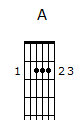
\includegraphics[scale=1.5]{../Akordy/a.png}
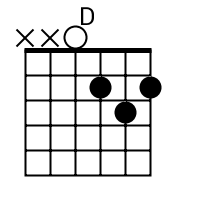
\includegraphics[scale=1.5]{../Akordy/d.png}
\end{figure}
